

\tikzset{every picture/.style={line width=0.75pt}} %set default line width to 0.75pt        

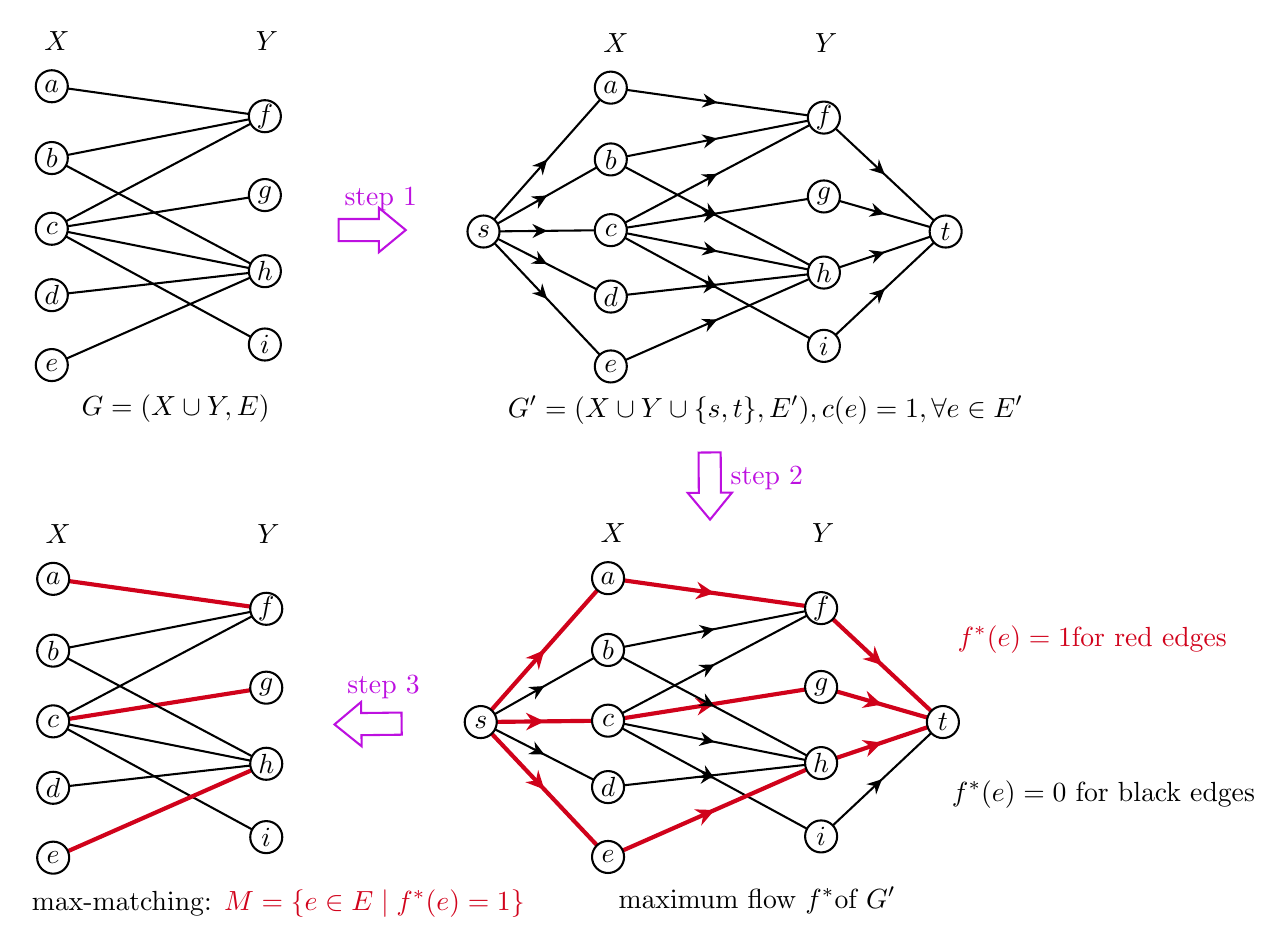
\begin{tikzpicture}[x=0.5pt,y=0.5pt,yscale=-1,xscale=1]
%uncomment if require: \path (0,664); %set diagram left start at 0, and has height of 664

%Straight Lines [id:da9104884328106918] 
\draw    (423.68,49.09) -- (331.68,153.07) ;
\draw [shift={(377.68,101.08)}, rotate = 131.5] [fill={rgb, 255:red, 0; green, 0; blue, 0 }  ][line width=0.08]  [draw opacity=0] (10.72,-5.15) -- (0,0) -- (10.72,5.15) -- (7.12,0) -- cycle    ;
%Straight Lines [id:da7681874141811359] 
\draw    (423.68,100.97) -- (331.68,153.07) ;
\draw [shift={(377.68,127.02)}, rotate = 150.48] [fill={rgb, 255:red, 0; green, 0; blue, 0 }  ][line width=0.08]  [draw opacity=0] (10.72,-5.15) -- (0,0) -- (10.72,5.15) -- (7.12,0) -- cycle    ;
%Straight Lines [id:da7226320448766448] 
\draw    (423.68,152.07) -- (331.68,153.07) ;
\draw [shift={(377.68,152.57)}, rotate = 179.38] [fill={rgb, 255:red, 0; green, 0; blue, 0 }  ][line width=0.08]  [draw opacity=0] (10.72,-5.15) -- (0,0) -- (10.72,5.15) -- (7.12,0) -- cycle    ;
%Straight Lines [id:da49080721425324236] 
\draw    (423.68,200.07) -- (331.68,153.07) ;
\draw [shift={(377.68,176.57)}, rotate = 207.06] [fill={rgb, 255:red, 0; green, 0; blue, 0 }  ][line width=0.08]  [draw opacity=0] (10.72,-5.15) -- (0,0) -- (10.72,5.15) -- (7.12,0) -- cycle    ;
%Straight Lines [id:da47091521890310684] 
\draw    (423.68,250.58) -- (331.68,153.07) ;
\draw [shift={(377.68,201.82)}, rotate = 226.66] [fill={rgb, 255:red, 0; green, 0; blue, 0 }  ][line width=0.08]  [draw opacity=0] (10.72,-5.15) -- (0,0) -- (10.72,5.15) -- (7.12,0) -- cycle    ;
%Straight Lines [id:da15266436710879794] 
\draw    (665.68,153.07) -- (577.67,70.73) ;
\draw [shift={(621.67,111.9)}, rotate = 223.09] [fill={rgb, 255:red, 0; green, 0; blue, 0 }  ][line width=0.08]  [draw opacity=0] (10.72,-5.15) -- (0,0) -- (10.72,5.15) -- (7.12,0) -- cycle    ;
%Straight Lines [id:da0877880561036608] 
\draw    (665.68,153.07) -- (577.67,127.73) ;
\draw [shift={(621.67,140.4)}, rotate = 196.06] [fill={rgb, 255:red, 0; green, 0; blue, 0 }  ][line width=0.08]  [draw opacity=0] (10.72,-5.15) -- (0,0) -- (10.72,5.15) -- (7.12,0) -- cycle    ;
%Straight Lines [id:da1013780616185066] 
\draw    (665.68,153.07) -- (577.67,182.73) ;
\draw [shift={(621.67,167.9)}, rotate = 161.38] [fill={rgb, 255:red, 0; green, 0; blue, 0 }  ][line width=0.08]  [draw opacity=0] (10.72,-5.15) -- (0,0) -- (10.72,5.15) -- (7.12,0) -- cycle    ;
%Straight Lines [id:da6251395403106741] 
\draw    (665.68,153.07) -- (577.67,235.73) ;
\draw [shift={(621.67,194.4)}, rotate = 136.8] [fill={rgb, 255:red, 0; green, 0; blue, 0 }  ][line width=0.08]  [draw opacity=0] (10.72,-5.15) -- (0,0) -- (10.72,5.15) -- (7.12,0) -- cycle    ;
%Straight Lines [id:da6233481480623783] 
\draw    (173.67,69.73) -- (19.68,99.97) ;
%Straight Lines [id:da3790939323014558] 
\draw    (19.68,48.09) -- (173.67,69.73) ;
%Straight Lines [id:da555393377892622] 
\draw    (173.67,69.73) -- (19.68,151.07) ;
%Straight Lines [id:da17109149534540602] 
\draw    (173.67,181.73) -- (19.68,151.07) ;
%Straight Lines [id:da8491552224613422] 
\draw    (173.67,234.73) -- (19.68,151.07) ;
%Straight Lines [id:da6111412207445381] 
\draw    (173.67,126.73) -- (19.68,151.07) ;
%Straight Lines [id:da40246334963984653] 
\draw    (173.67,181.73) -- (19.68,199.07) ;
%Straight Lines [id:da8951096474536266] 
\draw    (173.67,181.73) -- (19.68,249.58) ;
%Straight Lines [id:da442507224234595] 
\draw    (173.67,181.73) -- (19.68,99.97) ;
%Shape: Ellipse [id:dp9133580928774087] 
\draw  [fill={rgb, 255:red, 255; green, 255; blue, 255 }  ,fill opacity=1 ] (8.1,249.58) .. controls (8.1,243.18) and (13.29,238) .. (19.68,238) .. controls (26.08,238) and (31.26,243.18) .. (31.26,249.58) .. controls (31.26,255.97) and (26.08,261.16) .. (19.68,261.16) .. controls (13.29,261.16) and (8.1,255.97) .. (8.1,249.58) -- cycle ;
%Shape: Ellipse [id:dp4005957609675306] 
\draw  [fill={rgb, 255:red, 255; green, 255; blue, 255 }  ,fill opacity=1 ] (8.1,99.97) .. controls (8.1,93.57) and (13.29,88.39) .. (19.68,88.39) .. controls (26.08,88.39) and (31.26,93.57) .. (31.26,99.97) .. controls (31.26,106.36) and (26.08,111.55) .. (19.68,111.55) .. controls (13.29,111.55) and (8.1,106.36) .. (8.1,99.97) -- cycle ;
%Shape: Ellipse [id:dp49214617921702164] 
\draw  [fill={rgb, 255:red, 255; green, 255; blue, 255 }  ,fill opacity=1 ] (8.1,151.07) .. controls (8.1,144.67) and (13.29,139.49) .. (19.68,139.49) .. controls (26.08,139.49) and (31.26,144.67) .. (31.26,151.07) .. controls (31.26,157.46) and (26.08,162.65) .. (19.68,162.65) .. controls (13.29,162.65) and (8.1,157.46) .. (8.1,151.07) -- cycle ;
%Shape: Ellipse [id:dp8440754424343925] 
\draw  [fill={rgb, 255:red, 255; green, 255; blue, 255 }  ,fill opacity=1 ] (8.1,199.07) .. controls (8.1,192.68) and (13.29,187.49) .. (19.68,187.49) .. controls (26.08,187.49) and (31.26,192.68) .. (31.26,199.07) .. controls (31.26,205.47) and (26.08,210.65) .. (19.68,210.65) .. controls (13.29,210.65) and (8.1,205.47) .. (8.1,199.07) -- cycle ;
%Shape: Ellipse [id:dp20660183368429152] 
\draw  [fill={rgb, 255:red, 255; green, 255; blue, 255 }  ,fill opacity=1 ] (8.1,48.09) .. controls (8.1,41.7) and (13.29,36.51) .. (19.68,36.51) .. controls (26.08,36.51) and (31.26,41.7) .. (31.26,48.09) .. controls (31.26,54.49) and (26.08,59.67) .. (19.68,59.67) .. controls (13.29,59.67) and (8.1,54.49) .. (8.1,48.09) -- cycle ;
%Shape: Ellipse [id:dp4098192910838151] 
\draw  [fill={rgb, 255:red, 255; green, 255; blue, 255 }  ,fill opacity=1 ] (162.09,69.73) .. controls (162.09,63.33) and (167.27,58.15) .. (173.67,58.15) .. controls (180.06,58.15) and (185.25,63.33) .. (185.25,69.73) .. controls (185.25,76.13) and (180.06,81.31) .. (173.67,81.31) .. controls (167.27,81.31) and (162.09,76.13) .. (162.09,69.73) -- cycle ;
%Shape: Ellipse [id:dp04818959761719954] 
\draw  [fill={rgb, 255:red, 255; green, 255; blue, 255 }  ,fill opacity=1 ] (162.09,126.73) .. controls (162.09,120.33) and (167.27,115.15) .. (173.67,115.15) .. controls (180.06,115.15) and (185.25,120.33) .. (185.25,126.73) .. controls (185.25,133.13) and (180.06,138.31) .. (173.67,138.31) .. controls (167.27,138.31) and (162.09,133.13) .. (162.09,126.73) -- cycle ;
%Shape: Ellipse [id:dp776083183452069] 
\draw  [fill={rgb, 255:red, 255; green, 255; blue, 255 }  ,fill opacity=1 ] (162.09,181.73) .. controls (162.09,175.33) and (167.27,170.15) .. (173.67,170.15) .. controls (180.06,170.15) and (185.25,175.33) .. (185.25,181.73) .. controls (185.25,188.13) and (180.06,193.31) .. (173.67,193.31) .. controls (167.27,193.31) and (162.09,188.13) .. (162.09,181.73) -- cycle ;
%Shape: Ellipse [id:dp943943166831801] 
\draw  [fill={rgb, 255:red, 255; green, 255; blue, 255 }  ,fill opacity=1 ] (162.09,234.73) .. controls (162.09,228.33) and (167.27,223.15) .. (173.67,223.15) .. controls (180.06,223.15) and (185.25,228.33) .. (185.25,234.73) .. controls (185.25,241.13) and (180.06,246.31) .. (173.67,246.31) .. controls (167.27,246.31) and (162.09,241.13) .. (162.09,234.73) -- cycle ;
%Straight Lines [id:da2316107627226749] 
\draw    (577.67,70.73) -- (423.68,100.97) ;
\draw [shift={(500.67,85.85)}, rotate = 168.89] [fill={rgb, 255:red, 0; green, 0; blue, 0 }  ][line width=0.08]  [draw opacity=0] (10.72,-5.15) -- (0,0) -- (10.72,5.15) -- (7.12,0) -- cycle    ;
%Straight Lines [id:da18627772384857166] 
\draw    (423.68,49.09) -- (577.67,70.73) ;
\draw [shift={(500.67,59.91)}, rotate = 188] [fill={rgb, 255:red, 0; green, 0; blue, 0 }  ][line width=0.08]  [draw opacity=0] (10.72,-5.15) -- (0,0) -- (10.72,5.15) -- (7.12,0) -- cycle    ;
%Straight Lines [id:da0577243134049511] 
\draw    (577.67,70.73) -- (423.68,152.07) ;
\draw [shift={(500.67,111.4)}, rotate = 152.16] [fill={rgb, 255:red, 0; green, 0; blue, 0 }  ][line width=0.08]  [draw opacity=0] (10.72,-5.15) -- (0,0) -- (10.72,5.15) -- (7.12,0) -- cycle    ;
%Straight Lines [id:da5892851585558246] 
\draw    (577.67,182.73) -- (423.68,152.07) ;
\draw [shift={(500.67,167.4)}, rotate = 191.26] [fill={rgb, 255:red, 0; green, 0; blue, 0 }  ][line width=0.08]  [draw opacity=0] (10.72,-5.15) -- (0,0) -- (10.72,5.15) -- (7.12,0) -- cycle    ;
%Straight Lines [id:da3983360233296235] 
\draw    (577.67,235.73) -- (423.68,152.07) ;
\draw [shift={(500.67,193.9)}, rotate = 208.52] [fill={rgb, 255:red, 0; green, 0; blue, 0 }  ][line width=0.08]  [draw opacity=0] (10.72,-5.15) -- (0,0) -- (10.72,5.15) -- (7.12,0) -- cycle    ;
%Straight Lines [id:da6135696831152091] 
\draw    (577.67,127.73) -- (423.68,152.07) ;
\draw [shift={(500.67,139.9)}, rotate = 171.02] [fill={rgb, 255:red, 0; green, 0; blue, 0 }  ][line width=0.08]  [draw opacity=0] (10.72,-5.15) -- (0,0) -- (10.72,5.15) -- (7.12,0) -- cycle    ;
%Straight Lines [id:da9672640821433086] 
\draw    (577.67,182.73) -- (423.68,200.07) ;
\draw [shift={(500.67,191.4)}, rotate = 173.57] [fill={rgb, 255:red, 0; green, 0; blue, 0 }  ][line width=0.08]  [draw opacity=0] (10.72,-5.15) -- (0,0) -- (10.72,5.15) -- (7.12,0) -- cycle    ;
%Straight Lines [id:da7832805423777587] 
\draw    (577.67,182.73) -- (423.68,250.58) ;
\draw [shift={(500.67,216.65)}, rotate = 156.22] [fill={rgb, 255:red, 0; green, 0; blue, 0 }  ][line width=0.08]  [draw opacity=0] (10.72,-5.15) -- (0,0) -- (10.72,5.15) -- (7.12,0) -- cycle    ;
%Straight Lines [id:da1526453815123745] 
\draw    (577.67,182.73) -- (423.68,100.97) ;
\draw [shift={(500.67,141.85)}, rotate = 207.97] [fill={rgb, 255:red, 0; green, 0; blue, 0 }  ][line width=0.08]  [draw opacity=0] (10.72,-5.15) -- (0,0) -- (10.72,5.15) -- (7.12,0) -- cycle    ;
%Shape: Ellipse [id:dp6654229458693389] 
\draw  [fill={rgb, 255:red, 255; green, 255; blue, 255 }  ,fill opacity=1 ] (412.1,250.58) .. controls (412.1,244.18) and (417.29,239) .. (423.68,239) .. controls (430.08,239) and (435.26,244.18) .. (435.26,250.58) .. controls (435.26,256.97) and (430.08,262.16) .. (423.68,262.16) .. controls (417.29,262.16) and (412.1,256.97) .. (412.1,250.58) -- cycle ;
%Shape: Ellipse [id:dp12431995068279444] 
\draw  [fill={rgb, 255:red, 255; green, 255; blue, 255 }  ,fill opacity=1 ] (412.1,100.97) .. controls (412.1,94.57) and (417.29,89.39) .. (423.68,89.39) .. controls (430.08,89.39) and (435.26,94.57) .. (435.26,100.97) .. controls (435.26,107.36) and (430.08,112.55) .. (423.68,112.55) .. controls (417.29,112.55) and (412.1,107.36) .. (412.1,100.97) -- cycle ;
%Shape: Ellipse [id:dp20588104884103686] 
\draw  [fill={rgb, 255:red, 255; green, 255; blue, 255 }  ,fill opacity=1 ] (412.1,152.07) .. controls (412.1,145.67) and (417.29,140.49) .. (423.68,140.49) .. controls (430.08,140.49) and (435.26,145.67) .. (435.26,152.07) .. controls (435.26,158.46) and (430.08,163.65) .. (423.68,163.65) .. controls (417.29,163.65) and (412.1,158.46) .. (412.1,152.07) -- cycle ;
%Shape: Ellipse [id:dp7769132906685045] 
\draw  [fill={rgb, 255:red, 255; green, 255; blue, 255 }  ,fill opacity=1 ] (412.1,200.07) .. controls (412.1,193.68) and (417.29,188.49) .. (423.68,188.49) .. controls (430.08,188.49) and (435.26,193.68) .. (435.26,200.07) .. controls (435.26,206.47) and (430.08,211.65) .. (423.68,211.65) .. controls (417.29,211.65) and (412.1,206.47) .. (412.1,200.07) -- cycle ;
%Shape: Ellipse [id:dp9884072609577427] 
\draw  [fill={rgb, 255:red, 255; green, 255; blue, 255 }  ,fill opacity=1 ] (412.1,49.09) .. controls (412.1,42.7) and (417.29,37.51) .. (423.68,37.51) .. controls (430.08,37.51) and (435.26,42.7) .. (435.26,49.09) .. controls (435.26,55.49) and (430.08,60.67) .. (423.68,60.67) .. controls (417.29,60.67) and (412.1,55.49) .. (412.1,49.09) -- cycle ;
%Shape: Ellipse [id:dp42354463997423675] 
\draw  [fill={rgb, 255:red, 255; green, 255; blue, 255 }  ,fill opacity=1 ] (566.09,70.73) .. controls (566.09,64.33) and (571.27,59.15) .. (577.67,59.15) .. controls (584.06,59.15) and (589.25,64.33) .. (589.25,70.73) .. controls (589.25,77.13) and (584.06,82.31) .. (577.67,82.31) .. controls (571.27,82.31) and (566.09,77.13) .. (566.09,70.73) -- cycle ;
%Shape: Ellipse [id:dp6229410956087476] 
\draw  [fill={rgb, 255:red, 255; green, 255; blue, 255 }  ,fill opacity=1 ] (566.09,127.73) .. controls (566.09,121.33) and (571.27,116.15) .. (577.67,116.15) .. controls (584.06,116.15) and (589.25,121.33) .. (589.25,127.73) .. controls (589.25,134.13) and (584.06,139.31) .. (577.67,139.31) .. controls (571.27,139.31) and (566.09,134.13) .. (566.09,127.73) -- cycle ;
%Shape: Ellipse [id:dp791442075919042] 
\draw  [fill={rgb, 255:red, 255; green, 255; blue, 255 }  ,fill opacity=1 ] (566.09,182.73) .. controls (566.09,176.33) and (571.27,171.15) .. (577.67,171.15) .. controls (584.06,171.15) and (589.25,176.33) .. (589.25,182.73) .. controls (589.25,189.13) and (584.06,194.31) .. (577.67,194.31) .. controls (571.27,194.31) and (566.09,189.13) .. (566.09,182.73) -- cycle ;
%Shape: Ellipse [id:dp004238859938154427] 
\draw  [fill={rgb, 255:red, 255; green, 255; blue, 255 }  ,fill opacity=1 ] (566.09,235.73) .. controls (566.09,229.33) and (571.27,224.15) .. (577.67,224.15) .. controls (584.06,224.15) and (589.25,229.33) .. (589.25,235.73) .. controls (589.25,242.13) and (584.06,247.31) .. (577.67,247.31) .. controls (571.27,247.31) and (566.09,242.13) .. (566.09,235.73) -- cycle ;
%Shape: Ellipse [id:dp22397680523687857] 
\draw  [fill={rgb, 255:red, 255; green, 255; blue, 255 }  ,fill opacity=1 ] (320.1,153.07) .. controls (320.1,146.67) and (325.29,141.49) .. (331.68,141.49) .. controls (338.08,141.49) and (343.26,146.67) .. (343.26,153.07) .. controls (343.26,159.46) and (338.08,164.65) .. (331.68,164.65) .. controls (325.29,164.65) and (320.1,159.46) .. (320.1,153.07) -- cycle ;
%Shape: Ellipse [id:dp24170948792038305] 
\draw  [fill={rgb, 255:red, 255; green, 255; blue, 255 }  ,fill opacity=1 ] (654.1,153.07) .. controls (654.1,146.67) and (659.29,141.49) .. (665.68,141.49) .. controls (672.08,141.49) and (677.26,146.67) .. (677.26,153.07) .. controls (677.26,159.46) and (672.08,164.65) .. (665.68,164.65) .. controls (659.29,164.65) and (654.1,159.46) .. (654.1,153.07) -- cycle ;
%Straight Lines [id:da23171082184898195] 
\draw [color={rgb, 255:red, 208; green, 2; blue, 27 }  ,draw opacity=1 ][line width=1.5]    (421.68,403.59) -- (329.68,507.57) ;
\draw [shift={(375.68,455.58)}, rotate = 131.5] [fill={rgb, 255:red, 208; green, 2; blue, 27 }  ,fill opacity=1 ][line width=0.08]  [draw opacity=0] (13.4,-6.43) -- (0,0) -- (13.4,6.44) -- (8.9,0) -- cycle    ;
%Straight Lines [id:da1252268455632385] 
\draw    (421.68,455.47) -- (329.68,507.57) ;
\draw [shift={(375.68,481.52)}, rotate = 150.48] [fill={rgb, 255:red, 0; green, 0; blue, 0 }  ][line width=0.08]  [draw opacity=0] (10.72,-5.15) -- (0,0) -- (10.72,5.15) -- (7.12,0) -- cycle    ;
%Straight Lines [id:da6412216879845671] 
\draw [color={rgb, 255:red, 208; green, 2; blue, 27 }  ,draw opacity=1 ][line width=1.5]    (421.68,506.57) -- (329.68,507.57) ;
\draw [shift={(375.68,507.07)}, rotate = 179.38] [fill={rgb, 255:red, 208; green, 2; blue, 27 }  ,fill opacity=1 ][line width=0.08]  [draw opacity=0] (13.4,-6.43) -- (0,0) -- (13.4,6.44) -- (8.9,0) -- cycle    ;
%Straight Lines [id:da05952152958408119] 
\draw    (421.68,554.57) -- (329.68,507.57) ;
\draw [shift={(375.68,531.07)}, rotate = 207.06] [fill={rgb, 255:red, 0; green, 0; blue, 0 }  ][line width=0.08]  [draw opacity=0] (10.72,-5.15) -- (0,0) -- (10.72,5.15) -- (7.12,0) -- cycle    ;
%Straight Lines [id:da039385801791374964] 
\draw [color={rgb, 255:red, 208; green, 2; blue, 27 }  ,draw opacity=1 ][line width=1.5]    (421.68,605.08) -- (329.68,507.57) ;
\draw [shift={(375.68,556.32)}, rotate = 226.66] [fill={rgb, 255:red, 208; green, 2; blue, 27 }  ,fill opacity=1 ][line width=0.08]  [draw opacity=0] (13.4,-6.43) -- (0,0) -- (13.4,6.44) -- (8.9,0) -- cycle    ;
%Straight Lines [id:da38097100213841995] 
\draw [color={rgb, 255:red, 208; green, 2; blue, 27 }  ,draw opacity=1 ][line width=1.5]    (663.68,507.57) -- (575.67,425.23) ;
\draw [shift={(619.67,466.4)}, rotate = 223.09] [fill={rgb, 255:red, 208; green, 2; blue, 27 }  ,fill opacity=1 ][line width=0.08]  [draw opacity=0] (13.4,-6.43) -- (0,0) -- (13.4,6.44) -- (8.9,0) -- cycle    ;
%Straight Lines [id:da3947582528434521] 
\draw [color={rgb, 255:red, 208; green, 2; blue, 27 }  ,draw opacity=1 ][line width=1.5]    (663.68,507.57) -- (575.67,482.23) ;
\draw [shift={(619.67,494.9)}, rotate = 196.06] [fill={rgb, 255:red, 208; green, 2; blue, 27 }  ,fill opacity=1 ][line width=0.08]  [draw opacity=0] (13.4,-6.43) -- (0,0) -- (13.4,6.44) -- (8.9,0) -- cycle    ;
%Straight Lines [id:da1663751156591846] 
\draw [color={rgb, 255:red, 208; green, 2; blue, 27 }  ,draw opacity=1 ][line width=1.5]    (663.68,507.57) -- (575.67,537.23) ;
\draw [shift={(619.67,522.4)}, rotate = 161.38] [fill={rgb, 255:red, 208; green, 2; blue, 27 }  ,fill opacity=1 ][line width=0.08]  [draw opacity=0] (13.4,-6.43) -- (0,0) -- (13.4,6.44) -- (8.9,0) -- cycle    ;
%Straight Lines [id:da06142085666488806] 
\draw    (663.68,507.57) -- (575.67,590.23) ;
\draw [shift={(619.67,548.9)}, rotate = 136.8] [fill={rgb, 255:red, 0; green, 0; blue, 0 }  ][line width=0.08]  [draw opacity=0] (10.72,-5.15) -- (0,0) -- (10.72,5.15) -- (7.12,0) -- cycle    ;
%Straight Lines [id:da519880390315785] 
\draw    (575.67,425.23) -- (421.68,455.47) ;
\draw [shift={(498.67,440.35)}, rotate = 168.89] [fill={rgb, 255:red, 0; green, 0; blue, 0 }  ][line width=0.08]  [draw opacity=0] (10.72,-5.15) -- (0,0) -- (10.72,5.15) -- (7.12,0) -- cycle    ;
%Straight Lines [id:da9520097328287701] 
\draw [color={rgb, 255:red, 208; green, 2; blue, 27 }  ,draw opacity=1 ][line width=1.5]    (421.68,403.59) -- (575.67,425.23) ;
\draw [shift={(498.67,414.41)}, rotate = 188] [fill={rgb, 255:red, 208; green, 2; blue, 27 }  ,fill opacity=1 ][line width=0.08]  [draw opacity=0] (13.4,-6.43) -- (0,0) -- (13.4,6.44) -- (8.9,0) -- cycle    ;
%Straight Lines [id:da6291672599038822] 
\draw    (575.67,425.23) -- (421.68,506.57) ;
\draw [shift={(498.67,465.9)}, rotate = 152.16] [fill={rgb, 255:red, 0; green, 0; blue, 0 }  ][line width=0.08]  [draw opacity=0] (10.72,-5.15) -- (0,0) -- (10.72,5.15) -- (7.12,0) -- cycle    ;
%Straight Lines [id:da9636149434354304] 
\draw    (575.67,537.23) -- (421.68,506.57) ;
\draw [shift={(498.67,521.9)}, rotate = 191.26] [fill={rgb, 255:red, 0; green, 0; blue, 0 }  ][line width=0.08]  [draw opacity=0] (10.72,-5.15) -- (0,0) -- (10.72,5.15) -- (7.12,0) -- cycle    ;
%Straight Lines [id:da2766074901425193] 
\draw    (575.67,590.23) -- (421.68,506.57) ;
\draw [shift={(498.67,548.4)}, rotate = 208.52] [fill={rgb, 255:red, 0; green, 0; blue, 0 }  ][line width=0.08]  [draw opacity=0] (10.72,-5.15) -- (0,0) -- (10.72,5.15) -- (7.12,0) -- cycle    ;
%Straight Lines [id:da14316880527760267] 
\draw [color={rgb, 255:red, 208; green, 2; blue, 27 }  ,draw opacity=1 ][line width=1.5]    (575.67,482.23) -- (421.68,506.57) ;
\draw [shift={(498.67,494.4)}, rotate = 171.02] [fill={rgb, 255:red, 208; green, 2; blue, 27 }  ,fill opacity=1 ][line width=0.08]  [draw opacity=0] (13.4,-6.43) -- (0,0) -- (13.4,6.44) -- (8.9,0) -- cycle    ;
%Straight Lines [id:da7253343041193646] 
\draw    (575.67,537.23) -- (421.68,554.57) ;
\draw [shift={(498.67,545.9)}, rotate = 173.57] [fill={rgb, 255:red, 0; green, 0; blue, 0 }  ][line width=0.08]  [draw opacity=0] (10.72,-5.15) -- (0,0) -- (10.72,5.15) -- (7.12,0) -- cycle    ;
%Straight Lines [id:da6030254073421661] 
\draw [color={rgb, 255:red, 208; green, 2; blue, 27 }  ,draw opacity=1 ][line width=1.5]    (575.67,537.23) -- (421.68,605.08) ;
\draw [shift={(498.67,571.15)}, rotate = 156.22] [fill={rgb, 255:red, 208; green, 2; blue, 27 }  ,fill opacity=1 ][line width=0.08]  [draw opacity=0] (13.4,-6.43) -- (0,0) -- (13.4,6.44) -- (8.9,0) -- cycle    ;
%Straight Lines [id:da815770683078061] 
\draw    (575.67,537.23) -- (421.68,455.47) ;
\draw [shift={(498.67,496.35)}, rotate = 207.97] [fill={rgb, 255:red, 0; green, 0; blue, 0 }  ][line width=0.08]  [draw opacity=0] (10.72,-5.15) -- (0,0) -- (10.72,5.15) -- (7.12,0) -- cycle    ;
%Shape: Ellipse [id:dp6378572121821617] 
\draw  [fill={rgb, 255:red, 255; green, 255; blue, 255 }  ,fill opacity=1 ] (410.1,605.08) .. controls (410.1,598.68) and (415.29,593.5) .. (421.68,593.5) .. controls (428.08,593.5) and (433.26,598.68) .. (433.26,605.08) .. controls (433.26,611.47) and (428.08,616.66) .. (421.68,616.66) .. controls (415.29,616.66) and (410.1,611.47) .. (410.1,605.08) -- cycle ;
%Shape: Ellipse [id:dp28334771405699455] 
\draw  [fill={rgb, 255:red, 255; green, 255; blue, 255 }  ,fill opacity=1 ] (410.1,455.47) .. controls (410.1,449.07) and (415.29,443.89) .. (421.68,443.89) .. controls (428.08,443.89) and (433.26,449.07) .. (433.26,455.47) .. controls (433.26,461.86) and (428.08,467.05) .. (421.68,467.05) .. controls (415.29,467.05) and (410.1,461.86) .. (410.1,455.47) -- cycle ;
%Shape: Ellipse [id:dp2576705540128571] 
\draw  [fill={rgb, 255:red, 255; green, 255; blue, 255 }  ,fill opacity=1 ] (410.1,506.57) .. controls (410.1,500.17) and (415.29,494.99) .. (421.68,494.99) .. controls (428.08,494.99) and (433.26,500.17) .. (433.26,506.57) .. controls (433.26,512.96) and (428.08,518.15) .. (421.68,518.15) .. controls (415.29,518.15) and (410.1,512.96) .. (410.1,506.57) -- cycle ;
%Shape: Ellipse [id:dp8319819047488438] 
\draw  [fill={rgb, 255:red, 255; green, 255; blue, 255 }  ,fill opacity=1 ] (410.1,554.57) .. controls (410.1,548.18) and (415.29,542.99) .. (421.68,542.99) .. controls (428.08,542.99) and (433.26,548.18) .. (433.26,554.57) .. controls (433.26,560.97) and (428.08,566.15) .. (421.68,566.15) .. controls (415.29,566.15) and (410.1,560.97) .. (410.1,554.57) -- cycle ;
%Shape: Ellipse [id:dp7860831565588251] 
\draw  [fill={rgb, 255:red, 255; green, 255; blue, 255 }  ,fill opacity=1 ] (410.1,403.59) .. controls (410.1,397.2) and (415.29,392.01) .. (421.68,392.01) .. controls (428.08,392.01) and (433.26,397.2) .. (433.26,403.59) .. controls (433.26,409.99) and (428.08,415.17) .. (421.68,415.17) .. controls (415.29,415.17) and (410.1,409.99) .. (410.1,403.59) -- cycle ;
%Shape: Ellipse [id:dp15305882585242447] 
\draw  [fill={rgb, 255:red, 255; green, 255; blue, 255 }  ,fill opacity=1 ] (564.09,425.23) .. controls (564.09,418.83) and (569.27,413.65) .. (575.67,413.65) .. controls (582.06,413.65) and (587.25,418.83) .. (587.25,425.23) .. controls (587.25,431.63) and (582.06,436.81) .. (575.67,436.81) .. controls (569.27,436.81) and (564.09,431.63) .. (564.09,425.23) -- cycle ;
%Shape: Ellipse [id:dp4728125068549315] 
\draw  [fill={rgb, 255:red, 255; green, 255; blue, 255 }  ,fill opacity=1 ] (564.09,482.23) .. controls (564.09,475.83) and (569.27,470.65) .. (575.67,470.65) .. controls (582.06,470.65) and (587.25,475.83) .. (587.25,482.23) .. controls (587.25,488.63) and (582.06,493.81) .. (575.67,493.81) .. controls (569.27,493.81) and (564.09,488.63) .. (564.09,482.23) -- cycle ;
%Shape: Ellipse [id:dp8712157976640312] 
\draw  [fill={rgb, 255:red, 255; green, 255; blue, 255 }  ,fill opacity=1 ] (564.09,537.23) .. controls (564.09,530.83) and (569.27,525.65) .. (575.67,525.65) .. controls (582.06,525.65) and (587.25,530.83) .. (587.25,537.23) .. controls (587.25,543.63) and (582.06,548.81) .. (575.67,548.81) .. controls (569.27,548.81) and (564.09,543.63) .. (564.09,537.23) -- cycle ;
%Shape: Ellipse [id:dp5539674133813599] 
\draw  [fill={rgb, 255:red, 255; green, 255; blue, 255 }  ,fill opacity=1 ] (564.09,590.23) .. controls (564.09,583.83) and (569.27,578.65) .. (575.67,578.65) .. controls (582.06,578.65) and (587.25,583.83) .. (587.25,590.23) .. controls (587.25,596.63) and (582.06,601.81) .. (575.67,601.81) .. controls (569.27,601.81) and (564.09,596.63) .. (564.09,590.23) -- cycle ;
%Shape: Ellipse [id:dp49896351104083336] 
\draw  [fill={rgb, 255:red, 255; green, 255; blue, 255 }  ,fill opacity=1 ] (318.1,507.57) .. controls (318.1,501.17) and (323.29,495.99) .. (329.68,495.99) .. controls (336.08,495.99) and (341.26,501.17) .. (341.26,507.57) .. controls (341.26,513.96) and (336.08,519.15) .. (329.68,519.15) .. controls (323.29,519.15) and (318.1,513.96) .. (318.1,507.57) -- cycle ;
%Shape: Ellipse [id:dp4796257969400749] 
\draw  [fill={rgb, 255:red, 255; green, 255; blue, 255 }  ,fill opacity=1 ] (652.1,507.57) .. controls (652.1,501.17) and (657.29,495.99) .. (663.68,495.99) .. controls (670.08,495.99) and (675.26,501.17) .. (675.26,507.57) .. controls (675.26,513.96) and (670.08,519.15) .. (663.68,519.15) .. controls (657.29,519.15) and (652.1,513.96) .. (652.1,507.57) -- cycle ;
%Straight Lines [id:da6994945018285094] 
\draw    (174.67,425.73) -- (20.68,455.97) ;
%Straight Lines [id:da4790843187754682] 
\draw [color={rgb, 255:red, 208; green, 2; blue, 27 }  ,draw opacity=1 ][line width=1.5]    (20.68,404.09) -- (174.67,425.73) ;
%Straight Lines [id:da2359038596829396] 
\draw    (174.67,425.73) -- (20.68,507.07) ;
%Straight Lines [id:da33221605391600184] 
\draw    (174.67,537.73) -- (20.68,507.07) ;
%Straight Lines [id:da09840515113527637] 
\draw    (174.67,590.73) -- (20.68,507.07) ;
%Straight Lines [id:da393933721038044] 
\draw [color={rgb, 255:red, 208; green, 2; blue, 27 }  ,draw opacity=1 ][line width=1.5]    (174.67,482.73) -- (20.68,507.07) ;
%Straight Lines [id:da5874410168790086] 
\draw    (174.67,537.73) -- (20.68,555.07) ;
%Straight Lines [id:da1668343615235326] 
\draw [color={rgb, 255:red, 208; green, 2; blue, 27 }  ,draw opacity=1 ][line width=1.5]    (174.67,537.73) -- (20.68,605.58) ;
%Straight Lines [id:da18061979147739826] 
\draw    (174.67,537.73) -- (20.68,455.97) ;
%Shape: Ellipse [id:dp9525375874922476] 
\draw  [fill={rgb, 255:red, 255; green, 255; blue, 255 }  ,fill opacity=1 ] (9.1,605.58) .. controls (9.1,599.18) and (14.29,594) .. (20.68,594) .. controls (27.08,594) and (32.26,599.18) .. (32.26,605.58) .. controls (32.26,611.97) and (27.08,617.16) .. (20.68,617.16) .. controls (14.29,617.16) and (9.1,611.97) .. (9.1,605.58) -- cycle ;
%Shape: Ellipse [id:dp08180803888851007] 
\draw  [fill={rgb, 255:red, 255; green, 255; blue, 255 }  ,fill opacity=1 ] (9.1,455.97) .. controls (9.1,449.57) and (14.29,444.39) .. (20.68,444.39) .. controls (27.08,444.39) and (32.26,449.57) .. (32.26,455.97) .. controls (32.26,462.36) and (27.08,467.55) .. (20.68,467.55) .. controls (14.29,467.55) and (9.1,462.36) .. (9.1,455.97) -- cycle ;
%Shape: Ellipse [id:dp1440764994268804] 
\draw  [fill={rgb, 255:red, 255; green, 255; blue, 255 }  ,fill opacity=1 ] (9.1,507.07) .. controls (9.1,500.67) and (14.29,495.49) .. (20.68,495.49) .. controls (27.08,495.49) and (32.26,500.67) .. (32.26,507.07) .. controls (32.26,513.46) and (27.08,518.65) .. (20.68,518.65) .. controls (14.29,518.65) and (9.1,513.46) .. (9.1,507.07) -- cycle ;
%Shape: Ellipse [id:dp6045215355667296] 
\draw  [fill={rgb, 255:red, 255; green, 255; blue, 255 }  ,fill opacity=1 ] (9.1,555.07) .. controls (9.1,548.68) and (14.29,543.49) .. (20.68,543.49) .. controls (27.08,543.49) and (32.26,548.68) .. (32.26,555.07) .. controls (32.26,561.47) and (27.08,566.65) .. (20.68,566.65) .. controls (14.29,566.65) and (9.1,561.47) .. (9.1,555.07) -- cycle ;
%Shape: Ellipse [id:dp7390223184072033] 
\draw  [fill={rgb, 255:red, 255; green, 255; blue, 255 }  ,fill opacity=1 ] (9.1,404.09) .. controls (9.1,397.7) and (14.29,392.51) .. (20.68,392.51) .. controls (27.08,392.51) and (32.26,397.7) .. (32.26,404.09) .. controls (32.26,410.49) and (27.08,415.67) .. (20.68,415.67) .. controls (14.29,415.67) and (9.1,410.49) .. (9.1,404.09) -- cycle ;
%Shape: Ellipse [id:dp8156351680962495] 
\draw  [fill={rgb, 255:red, 255; green, 255; blue, 255 }  ,fill opacity=1 ] (163.09,425.73) .. controls (163.09,419.33) and (168.27,414.15) .. (174.67,414.15) .. controls (181.06,414.15) and (186.25,419.33) .. (186.25,425.73) .. controls (186.25,432.13) and (181.06,437.31) .. (174.67,437.31) .. controls (168.27,437.31) and (163.09,432.13) .. (163.09,425.73) -- cycle ;
%Shape: Ellipse [id:dp04933624666042746] 
\draw  [fill={rgb, 255:red, 255; green, 255; blue, 255 }  ,fill opacity=1 ] (163.09,482.73) .. controls (163.09,476.33) and (168.27,471.15) .. (174.67,471.15) .. controls (181.06,471.15) and (186.25,476.33) .. (186.25,482.73) .. controls (186.25,489.13) and (181.06,494.31) .. (174.67,494.31) .. controls (168.27,494.31) and (163.09,489.13) .. (163.09,482.73) -- cycle ;
%Shape: Ellipse [id:dp018734192435295283] 
\draw  [fill={rgb, 255:red, 255; green, 255; blue, 255 }  ,fill opacity=1 ] (163.09,537.73) .. controls (163.09,531.33) and (168.27,526.15) .. (174.67,526.15) .. controls (181.06,526.15) and (186.25,531.33) .. (186.25,537.73) .. controls (186.25,544.13) and (181.06,549.31) .. (174.67,549.31) .. controls (168.27,549.31) and (163.09,544.13) .. (163.09,537.73) -- cycle ;
%Shape: Ellipse [id:dp44298738112423197] 
\draw  [fill={rgb, 255:red, 255; green, 255; blue, 255 }  ,fill opacity=1 ] (163.09,590.73) .. controls (163.09,584.33) and (168.27,579.15) .. (174.67,579.15) .. controls (181.06,579.15) and (186.25,584.33) .. (186.25,590.73) .. controls (186.25,597.13) and (181.06,602.31) .. (174.67,602.31) .. controls (168.27,602.31) and (163.09,597.13) .. (163.09,590.73) -- cycle ;
%Right Arrow [id:dp48750820094256064] 
\draw  [color={rgb, 255:red, 189; green, 16; blue, 224 }  ,draw opacity=1 ] (227,144) -- (256.1,144) -- (256.1,136) -- (275.5,152) -- (256.1,168) -- (256.1,160) -- (227,160) -- cycle ;
%Right Arrow [id:dp7632701021121623] 
\draw  [color={rgb, 255:red, 189; green, 16; blue, 224 }  ,draw opacity=1 ] (272.59,516.71) -- (243.5,517.06) -- (243.59,525.06) -- (224,509.29) -- (243.21,493.06) -- (243.3,501.06) -- (272.4,500.71) -- cycle ;
%Right Arrow [id:dp021626154346667814] 
\draw  [color={rgb, 255:red, 189; green, 16; blue, 224 }  ,draw opacity=1 ] (503.08,312.69) -- (503.28,341.79) -- (511.28,341.74) -- (495.42,361.25) -- (479.28,341.96) -- (487.28,341.91) -- (487.08,312.81) -- cycle ;

% Text Node
\draw (19.68,249.58) node   [align=left] {$\displaystyle e$};
% Text Node
\draw (19.68,99.97) node   [align=left] {$\displaystyle b$};
% Text Node
\draw (19.68,151.07) node   [align=left] {$\displaystyle c$};
% Text Node
\draw (19.68,199.07) node   [align=left] {$\displaystyle d$};
% Text Node
\draw (19.68,48.09) node   [align=left] {$\displaystyle a$};
% Text Node
\draw (173.67,69.73) node   [align=left] {$\displaystyle f$};
% Text Node
\draw (39,268.5) node [anchor=north west][inner sep=0.75pt]   [align=left] {$\displaystyle G=( X\cup Y,E)$};
% Text Node
\draw (173.67,126.73) node   [align=left] {$\displaystyle g$};
% Text Node
\draw (173.67,181.73) node   [align=left] {$\displaystyle h$};
% Text Node
\draw (173.67,234.73) node   [align=left] {$\displaystyle i$};
% Text Node
\draw (12,6.5) node [anchor=north west][inner sep=0.75pt]   [align=left] {$\displaystyle X$};
% Text Node
\draw (165,6.5) node [anchor=north west][inner sep=0.75pt]   [align=left] {$\displaystyle Y$};
% Text Node
\draw (423.68,250.58) node   [align=left] {$\displaystyle e$};
% Text Node
\draw (423.68,100.97) node   [align=left] {$\displaystyle b$};
% Text Node
\draw (423.68,152.07) node   [align=left] {$\displaystyle c$};
% Text Node
\draw (423.68,200.07) node   [align=left] {$\displaystyle d$};
% Text Node
\draw (423.68,49.09) node   [align=left] {$\displaystyle a$};
% Text Node
\draw (577.67,70.73) node   [align=left] {$\displaystyle f$};
% Text Node
\draw (347,269.5) node [anchor=north west][inner sep=0.75pt]   [align=left] {$\displaystyle G'=( X\cup Y\cup \{s,t\} ,E') ,c( e) =1,\forall e\in E'$};
% Text Node
\draw (577.67,127.73) node   [align=left] {$\displaystyle g$};
% Text Node
\draw (577.67,182.73) node   [align=left] {$\displaystyle h$};
% Text Node
\draw (577.67,235.73) node   [align=left] {$\displaystyle i$};
% Text Node
\draw (416,7.5) node [anchor=north west][inner sep=0.75pt]   [align=left] {$\displaystyle X$};
% Text Node
\draw (569,7.5) node [anchor=north west][inner sep=0.75pt]   [align=left] {$\displaystyle Y$};
% Text Node
\draw (331.68,153.07) node   [align=left] {$\displaystyle s$};
% Text Node
\draw (665.68,153.07) node   [align=left] {$\displaystyle t$};
% Text Node
\draw (421.68,605.08) node   [align=left] {$\displaystyle e$};
% Text Node
\draw (421.68,455.47) node   [align=left] {$\displaystyle b$};
% Text Node
\draw (421.68,506.57) node   [align=left] {$\displaystyle c$};
% Text Node
\draw (421.68,554.57) node   [align=left] {$\displaystyle d$};
% Text Node
\draw (421.68,403.59) node   [align=left] {$\displaystyle a$};
% Text Node
\draw (575.67,425.23) node   [align=left] {$\displaystyle f$};
% Text Node
\draw (427,624) node [anchor=north west][inner sep=0.75pt]   [align=left] {maximum flow $\displaystyle f^{*}$of $\displaystyle G'$};
% Text Node
\draw (575.67,482.23) node   [align=left] {$\displaystyle g$};
% Text Node
\draw (575.67,537.23) node   [align=left] {$\displaystyle h$};
% Text Node
\draw (575.67,590.23) node   [align=left] {$\displaystyle i$};
% Text Node
\draw (414,362) node [anchor=north west][inner sep=0.75pt]   [align=left] {$\displaystyle X$};
% Text Node
\draw (567,362) node [anchor=north west][inner sep=0.75pt]   [align=left] {$\displaystyle Y$};
% Text Node
\draw (329.68,507.57) node   [align=left] {$\displaystyle s$};
% Text Node
\draw (663.68,507.57) node   [align=left] {$\displaystyle t$};
% Text Node
\draw (20.68,605.58) node   [align=left] {$\displaystyle e$};
% Text Node
\draw (20.68,455.97) node   [align=left] {$\displaystyle b$};
% Text Node
\draw (20.68,507.07) node   [align=left] {$\displaystyle c$};
% Text Node
\draw (20.68,555.07) node   [align=left] {$\displaystyle d$};
% Text Node
\draw (20.68,404.09) node   [align=left] {$\displaystyle a$};
% Text Node
\draw (174.67,425.73) node   [align=left] {$\displaystyle f$};
% Text Node
\draw (3,626.5) node [anchor=north west][inner sep=0.75pt]   [align=left] {max-matching: $\displaystyle \textcolor[rgb]{0.82,0.01,0.11}{M=\left\{e\in E\mid f^{*}( e) =1\right\}}$};
% Text Node
\draw (174.67,482.73) node   [align=left] {$\displaystyle g$};
% Text Node
\draw (174.67,537.73) node   [align=left] {$\displaystyle h$};
% Text Node
\draw (174.67,590.73) node   [align=left] {$\displaystyle i$};
% Text Node
\draw (13,362.5) node [anchor=north west][inner sep=0.75pt]   [align=left] {$\displaystyle X$};
% Text Node
\draw (166,362.5) node [anchor=north west][inner sep=0.75pt]   [align=left] {$\displaystyle Y$};
% Text Node
\draw (229,119) node [anchor=north west][inner sep=0.75pt]  [color={rgb, 255:red, 189; green, 16; blue, 224 }  ,opacity=1 ] [align=left] {step 1};
% Text Node
\draw (231,472) node [anchor=north west][inner sep=0.75pt]  [color={rgb, 255:red, 189; green, 16; blue, 224 }  ,opacity=1 ] [align=left] {step 3};
% Text Node
\draw (508,321) node [anchor=north west][inner sep=0.75pt]  [color={rgb, 255:red, 189; green, 16; blue, 224 }  ,opacity=1 ] [align=left] {step 2};
% Text Node
\draw (672,436) node [anchor=north west][inner sep=0.75pt]   [align=left] {\textcolor[rgb]{0.82,0.01,0.11}{$\displaystyle f^{*}( e) =1$}\textcolor[rgb]{0.82,0.01,0.11}{ for red edges}};
% Text Node
\draw (668,548) node [anchor=north west][inner sep=0.75pt]   [align=left] {$\displaystyle f^{*}( e) =0$ for black edges};


\end{tikzpicture}

